\documentclass[10pt]{article}
\usepackage[slovene]{babel}
\usepackage[utf8]{inputenc}
\usepackage[T2A]{fontenc}
\usepackage{amsmath}
\usepackage{amsfonts}
\usepackage{amssymb}
\usepackage[version=4]{mhchem}
\usepackage{stmaryrd}
\usepackage{graphicx}
\usepackage[export]{adjustbox}
\graphicspath{ {./images/} }
\usepackage{physics}
\usepackage{geometry}
\geometry{left=2cm,right=2cm,top=2cm,bottom=2cm}



\title{Sevanje črnega telesa}
\author{Samo Krejan}
\date{marec 2025}


\begin{document}
\maketitle

\section{Uvod}

Gostoto energije elektromagnetnega valovanja z neko frekvenco $\nu$ v votlini pri temperaturi $T$ določa Planckova formula \ref{planck}.

\begin{equation}
    w(\nu, T) = \frac{8\pi h \nu^3}{c^3} \frac{1}{\exp(h\nu/kT) -1},
    \label{planck}
\end{equation}
kjer je $h$ Planckova konstanta in $c$ hitrost svetlobe v vakumu. Če v tako votlino naredimo majhno luknjico je to kar najboljši približek sevanja črnega telesa. Gostota energijskega toka skozi tako luknjico je \ref{gostota}:

\begin{equation}
    j(\nu, T) = \frac{1}{4} c w(\nu,T)
    \label{gostota}
\end{equation}
Svetloba ki seva iz luknjice sledi Lambertovem kosinusnem zakonu (intenziteta je sorazmerna s kosinusom kota pod katerim opazujemo). Tudi volframska nitka v žarnici je dober približek črnega telesa, kot je tudi sonce, ki seva kot črno telo pri temperaturi $5800\ K$. S to vajo bomo merili sevanje volframske nitke v halogenski žarnici, ki ji lahko spreminjamo temperaturo v zelo širokem obsegu. Z absolutnim merilnikom sevanja bomo določili celoten energijski tok, ki ga seva žarnica in ga nato primerjali z močjo, ki jo troši.


\section{Naloga}

\begin{itemize}
    \item Izmerite odvisnost svetlobnega toka halogenske žarnice v razponu od rahlega žarjenja do maksimalne moči. Pri tem merite tudi moč, ki se troši na žarnici,
    \item narišite graf celotne izsevane moči kot funkcijo izsevane moči,
    \item določite električno upornost žarnice kot funkcijo temperature,
    \item narišite graf razmerja med - skozi $Si$ okno - prepuščenim in nemotenim svetlobnim tokom kot funkcijo temperature žarilne nitke.
\end{itemize}


\section{Potrebščine}

\begin{itemize}
    \item Merilec električne moči (wattmeter) in električni multimeter,
    \item halogenska žarnica nazivne moči $30W$ z nazivno barvno temperaturo $2700K$,
    \item nastavljivi transformator - variac,
    \item merilnik sevanja,
    \item plošča iz kristalnega silicija.
\end{itemize}

\section{Rezultati in analiza}

Najprej smo izmerili upor žarnice ko je bila ugasnjena. To smo storili z multimetrom, ki je pokazal vrednost $120\ \Omega \pm 1\ \Omega$. Odčitali smo tudi razdaljo med žarnico in senzorejem. Ta je znašala $d = 29,5\ cm \pm 0,5\ cm$.

Moč ozadja smo izmerili, tako da smo postavili ščit pred žarnico, pri petih različnih močeh žarnice in dobili: $P_{ozadje} = (-20\pm 20)\ \mu W$. Negativne vrednosti nas malo zaskrbijo, saj bi to lahko pomenilo, da stvari niso dobro kalibrirane, a se s tem ne ukvarjamo dosti, saj so vrednosti ozadja praktično nič.

\bigskip

\noindent Vrednosti ozadja lahko sedaj odštejemo od ostalih izmerjenih vrednosti in nato ustrezno izračunamo celotno moč, ki jo izseva žarnica. To naredimo po enačbi \ref{cela moč}

\begin{equation}
    P_{cela} = P_{izmerjena} \frac{4\pi d^2}{S_0}
    \label{cela moč}
\end{equation}
kjer je $S_0 = 0,71\ cm^2$ površina senzorja podana v navodilih. Podatke predstavimo v tabeli \ref{moči}:

\begin{table}[!ht]
    \centering
    \begin{tabular}{l|l|l|l}
        $P_{i,b}$ & $P_{i,si}$ & $P_{c,b}$ & $P_{c,si}$ \\ \hline
        0.0 & -2e-05 & 0.0 & -0.30805 \\ 
        6e-05 & 2e-05 & 0.92416 & 0.30805 \\ 
        0.00017 & 8e-05 & 2.61845 & 1.23221 \\ 
        0.0003 & 0.00014 & 4.6208 & 2.15637 \\ 
        0.00047 & 0.00022 & 7.23925 & 3.38858 \\ 
        0.00065 & 0.0003 & 10.01172 & 4.6208 \\ 
        0.00076 & 0.00034 & 11.70602 & 5.2369 \\ 
        0.00088 & 0.00041 & 13.55434 & 6.31509 \\ 
        0.001 & 0.00043 & 15.40265 & 6.62314 \\ 
        0.00118 & 0.00052 & 18.17513 & 8.00938 \\ 
        0.00131 & 0.00056 & 20.17748 & 8.62549 \\ 
        0.00142 & 0.00062 & 21.87177 & 9.54965 \\ 
        0.00158 & 0.00066 & 24.33619 & 10.16575 \\ 
        0.00174 & 0.00072 & 26.80062 & 11.08991 \\ 
        0.00188 & 0.00077 & 28.95699 & 11.86004 \\ 
        0.00211 & 0.00084 & 32.4996 & 12.93823 \\ 
        0.00223 & 0.00086 & 34.34792 & 13.24628 \\ 
        0.00239 & 0.00092 & 36.81234 & 14.17044 \\ 
        0.00242 & 0.00094 & 37.27442 & 14.47849 \\ 
    \end{tabular}
    \caption{Tabela izmerjenih in preračunanih moči brez in z Silicijevega zaslona}
    \label{moči}
\end{table}

\noindent Podatki so predstavljeni brez napak, lahko pa le te precej dobro ocenimo na $5\%$, $3,5$ zaradi napake pri merjenju razdalje (in njenem kvadriranju), ter $1,5$ zaradi napake pri merjenju moči. Napaka variira okoli te vrednosti a $5\%$ je zgornja meja.

Zdaj, ko smo to poračunali, lahko primerjamo celotno izsevano moč $P_{c,b}$ in električno moč, ki smo jo tudi merili. Te predstavimo na grafu \ref{izkoristek} skupaj z grafom simetrale prvega kvadranta, ki predstavlja \textit{idealen izkoristek}.

Vidimo lahko, da se podatki ne prilegajo popolnoma premici, za kar je morda res kriva neka sistemska napaka v merilcu svetlobnega toka, ali pa se nekaj moči izgubi na poti od žarnice do senzorja zaradi stekla ali pa zraka, čeprav mi fizikalna intuicija pravi, da so take izgube res minimalne. Še dodatno pojasnilo je, da se del moči porabi tudi na tokokrogu pred žarnico.

\begin{figure}[ht]
\begin{center}
    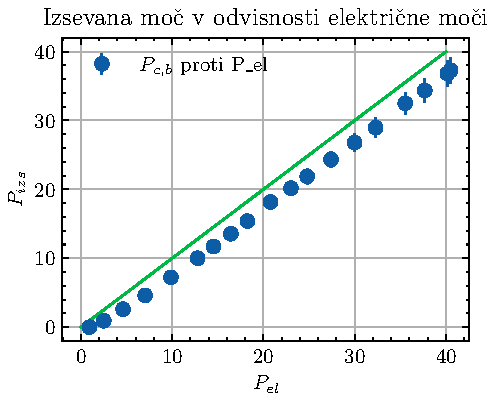
\includegraphics[width=8cm]{izkoristek.pdf}
    \caption{Celotna izsevana moč v odvisnosti od električne moči}
    \label{izkoristek}
\end{center}
\end{figure}

\newpage

Upornost žarnice izračunamo preprosto kot $R = U/I$ pri računanju temperature pa imamo malo več dela. Samo Štefanov zakon ne zadostuje,saj nimamo podatka o površini žarilne nitke. Lahko pa se opremo na dejstvo, da je ta konstantna in je tako konstantno tudi razmerje $T^4/P$. Ko to združimo s podatkom, da ima žarnica pri nazivni moči $P_0 = 30\ W$ temperaturo $T_0=2700\ K$ lahko nadaljno temperaturo računamo kot po enačbi \ref{temp}:

\begin{equation}
    T = T_0 \sqrt[4]{\frac{P}{P_0}}
    \label{temp}
\end{equation}
S pomočjo teh dveh formul lahko izračunamo upor v odvisnosti od izsevane moči in preverimo, če je odvisnost res linearna. Izračunane podatke prikažemo na grafu \ref{upor}:

\begin{figure}[ht]
\begin{center}
    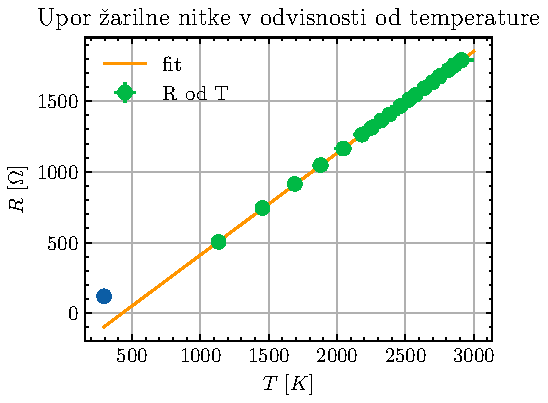
\includegraphics[width=8cm]{upor.pdf}
    \caption{Upor v odvisnosti od temperature}
    \label{upor}
\end{center}
\end{figure}

\noindent Vidimo lahko, da je odvisnost res linearna. Edina točka, ki odstopa od meritev je upor žarnice pri sobni temperaturi. Razlogov za to je seveda več, lahko da je prišlo spet do sistemske napake pri meritvi moči, kot smo diskutirali že pri primerjavi izsevane in električne moči, lahko pa da nismo merili le upora žarnice, pač pa tudi ohišja.

Linearno odvisnost upora in temperature lahko opišemo z enačbo \ref{lin-upor}:

\begin{equation}
    R = m T + b
    \label{lin-upor}
\end{equation}
kjer smo s Pythonom odčitali $m = 0.720\ \Omega /K$ in $b = -308.5\ \Omega$. Predvsem vrednost $b$ nam da misliti, da linearna odvisnost ne more veljati na širokem razponu temperatur.





\end{document}